\section{Introduction}

% single applicaiotn -> performance + power


The hardware nodes of a cloud service provider are often dedicated to running a single cloud service component~\cite{FB}. 
%todo: think about cite something, e.g., facebook citation, and figure out if they actually use dedicated nature to do both, in which case we can combine above and next sentance
One hopes that this dedicated nature (i.e. fixed role in the service using a fixed software stack) can be exploited to obtain the required performance (e.g. 99\% tail latency) while minimizing the energy used; a key concern given the increasingly constrained energy budgets in data centers~\cite{SmoothOperator, Dynamo, oldi}. 
%YA
%When we consider the performance and energy use of a system, it is critical to note that they are emergent properties of the myriad of interactions between application software, operating systems, hardware, and offered loads.
%However, if we then take a careful look at overall system execution under different energy profiles, we can see that the consequences of tuning energy and performance reach far beyond directly observable quantities and impact the interactions between the aforementioned system components in subtle ways.
%%However, the performance and energy use of a system is an emergent property of the myriad of interactions between application software, operating systems, and hardware along with the offered load. 
%%todo: above ends where, why is this a however?
%%As OS developers do we really understand what is going on and the impact of each of our decisions?
%Rather than focusing on the design and implementation of particular local or global mechanisms and policies for tuning performance and energy consumption, perhaps we need a greater understanding of their underlying impacts and dynamics.   

% we have been building a library OS, and wanted to figure out HW settings...
% this led us to a study
In this paper, we present findings from a  study of the emergent impact that server operating systems' design and implementation, as well as their interaction with hardware settings, can have on the combination of performance and energy when running a single application.
This study grew out of our effort on developing a bare-metal library OS ({\em libOS}).
%
%We ported our previously developed libOS to run on physical hardware  to study the possible impacts bare-metal library OS use could have on both performance and energy consumption.  
%See section~\cref{sec:exp_setup} for details regarding the NIC and our support for it.  
Given the prior use of our libOS in virtualized environments, we had no policies, neither static nor dynamic, for many hardware settings.  
The complexity of deciding what settings to use was daunting; we found that the NIC alone has thousands of registers that might impact performance or power.  
%%todo: Han, fix above sentance
%After some research and experimentation we identified the NICs interrupt delay register (ITR), processor sleep states, processor dynamic frequency and voltage scaling settings (DVFS) and package level power capacity limits (RAPL) to be of priority to explore. 


%We have
%studying bare-metal library OS ({\em libOS}) use for data-center workloads.
%While our particular libOS is designed for both virtual and bare-metal
%operation the majority of our experience had been studying it virtualized.  
%Once we completed a port of a more sophisticated standard Network Interface
%Card (NIC) we were in a position to more extensively study the possible impacts
%bare-metal library OS use could have on both performance and energy consumption.  
%See section~\cref{sec:exp_setup} for details regarding the NIC and our support
%for it.  
%However, we quickly realized that given the simple nature of our
%systems and pre-dominate prior use in virtualized environments, we had no
%policies, neither static nor dynamic for many hardware settings.  

%When designing and implementing an operating system there is a dizzying array of mechanisms and policies one must consider, both at a local and global scale, that could both individually and collaboratively impact the performance and energy use of the system.
%In this paper, we present findings from a detailed study on the impact of hardware tuning on the performance and energy consumption of applications running on top of two baremetal OSes with fundamentally different design and implementation.
%This study grew out of our efforts to explore a baremetal library OS (libOS) for running datacenter workloads.

Our first thought was to simply inherit the default values and policies that Linux uses for our same hardware platform.
%-- static defaults and the dominate or mean value for dynamically adjusted parameters when running the same workload. 
%We quickly discovered Linux's behaviour with respect to these setting was a
%complex mixture of dynamic and administrator controlled parameters.  
However, it soon became clear that the actual impact and optimality of Linux's defaults on the energy consumption and realized performance was not discernible though inspection and reasoning.  
%Nor was it clear, through causal reasoning, what Linux's behaviour would be when manually overriding the defaults with static values. 
As a result, we decided to pursue a detailed study that would explore the performance and energy use of both Linux and our system under a variety of hardware settings and workloads. 




%We were initially motivated by a desire to understand the significance of the default values of hardware settings used by Linux and their corresponding impact on the optimality of energy consumption and overall application performance.
%Moreover, when causal reasoning fell short, we were driven to explore, through experimental observation and analysis, Linux's behavior when manually overriding its default hardware tuning policies with statically tuned values.
%During this study, we required the libOS to inherit the default hardware settings that Linux uses for the same machine without fully understanding the actual impact and optimality of Linux's default settings on the energy consumption and on overall application performance. Nor was it clear through causal reasoning what Linux's behaviour would be when manually overriding its default policies with statically tuned values.

\begin{table}[t]
\centering
\begin{tabular}{l|c|c|c}
  Name & Scenarios & Nature & CPU\\
  \hline
  NetPIPE & {\small 64B,8KB,64KB,512KB} & CL & Low\\ \hline
  NodeJS & na & CL & High \\ \hline
  Memcached & 200K, 400K, 600K & OL & Low \\ \hline
  Silo & 50K, 100K, 200K & OL & High \\ 
\end{tabular}
\caption{Workload configurations. NetPIPE and NodeJS are single thread, single connection workloads. Memcached and Memcached-silo are multiple cores, multiple connection workloads. The column {\em nature} indicates if the workload is open or closed loop, and {\em CPU} indicates if there is a significant application compute involved on each request.}
\label{table:wrkcfgs}	
\end{table}



%We decided to focus our study on just three hardware settings (see \cref{sec:knobs}), namely: 1) Network Interface Card (NIC) Interrupt delay (ITR), 2) Dynamic Voltage and Frequency Scaling (DVFS) and 3) Running Average Power Limit (RAPL). 
%We chose ITR because of both its obvious importance to trade off latency versus throughput in network driven workloads, and the latter two because of their importance for reducing energy consumption.  
%
\begin{figure*}[thb]
\centering	
\begin{minipage}[t]{0.45\textwidth}
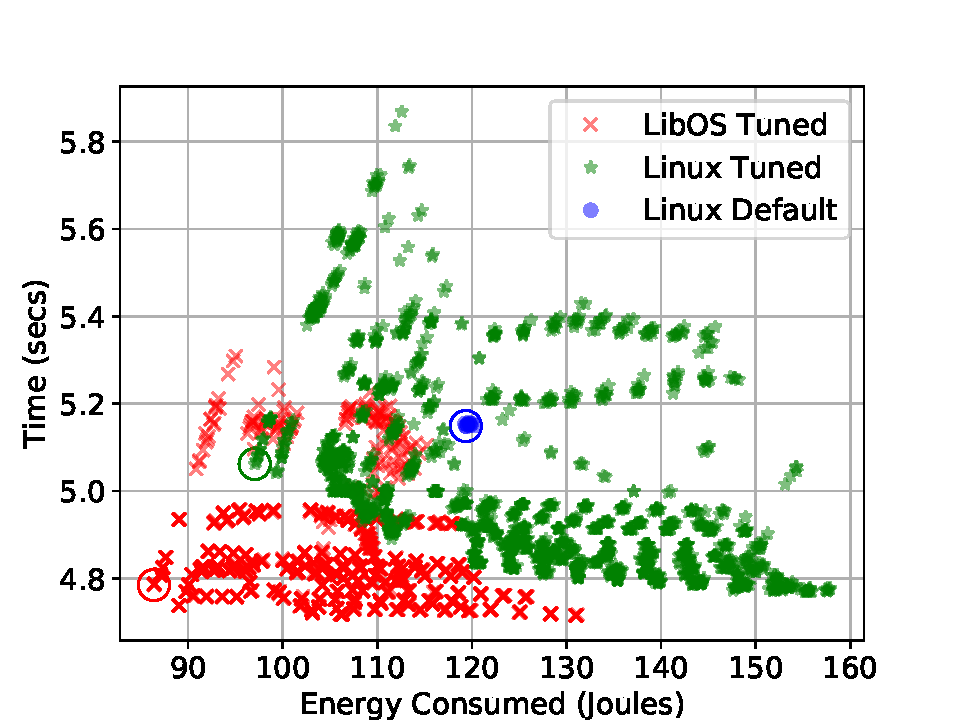
\includegraphics[width=\textwidth]{osdi_figures/netpipe_524288_overview.pdf}
	\caption{Netpipe 512 KB overview}
	\label{fig:netpipe8Kov}
\end{minipage}
\begin{minipage}[t]{0.45\textwidth}
	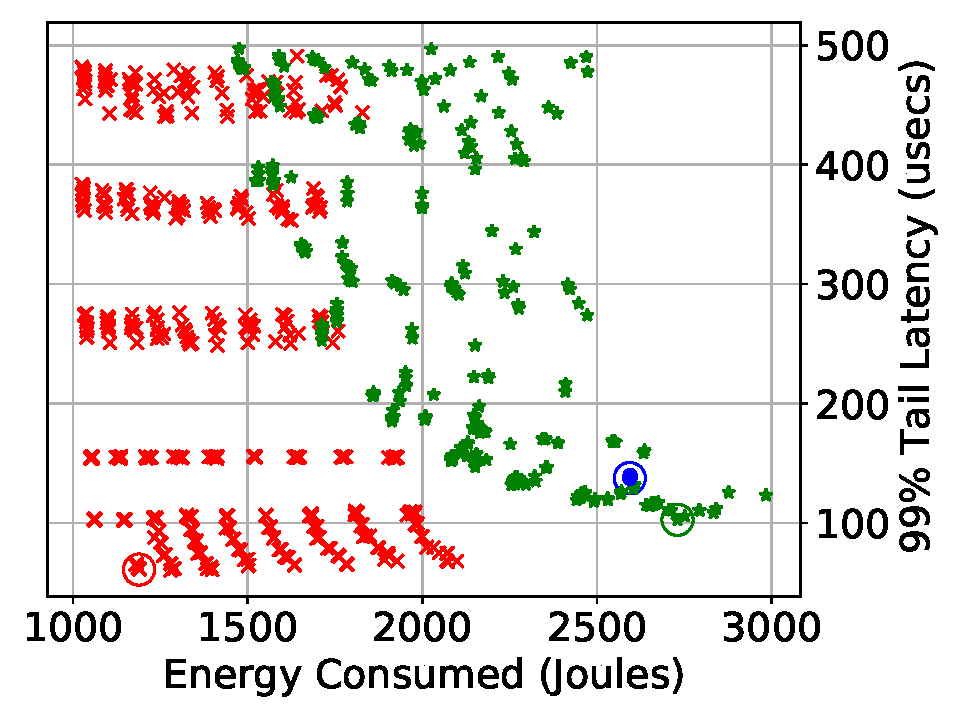
\includegraphics[width=\columnwidth]{osdi_figures/mcd_600000_overview.pdf}
	\caption{Memcached 600K QPS}
	\label{fig:mcdov}
\end{minipage}
\begin{minipage}[t]{0.45\textwidth}
	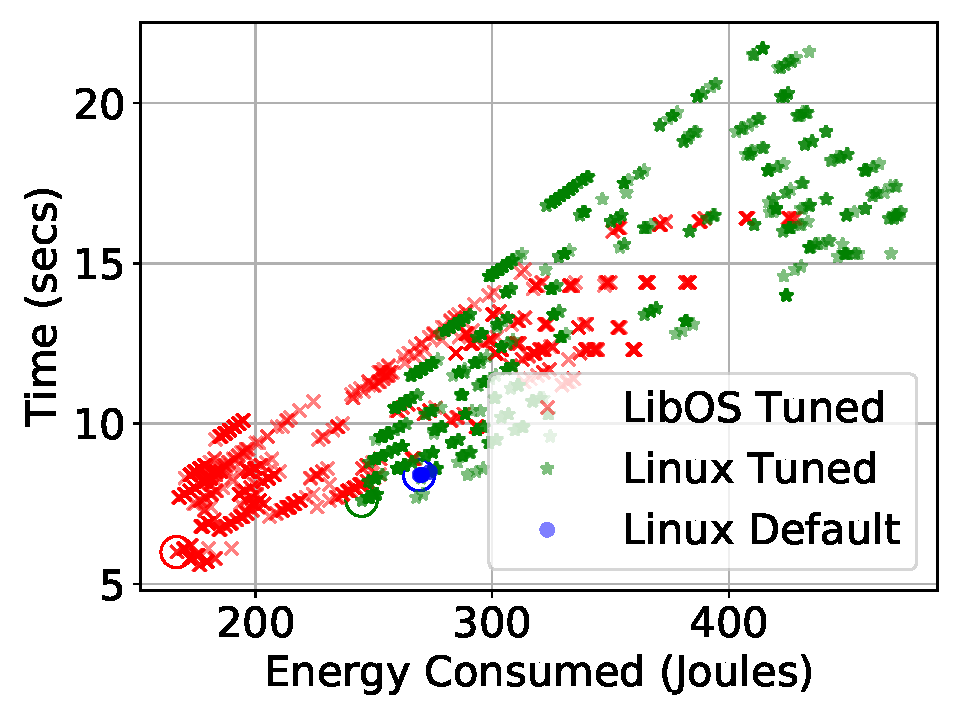
\includegraphics[width=\textwidth]{osdi_figures/nodejs_overview.pdf}
	\caption{NodeJS overview}
	\label{fig:nodejsov}
\end{minipage}
\begin{minipage}[t]{0.45\textwidth}
	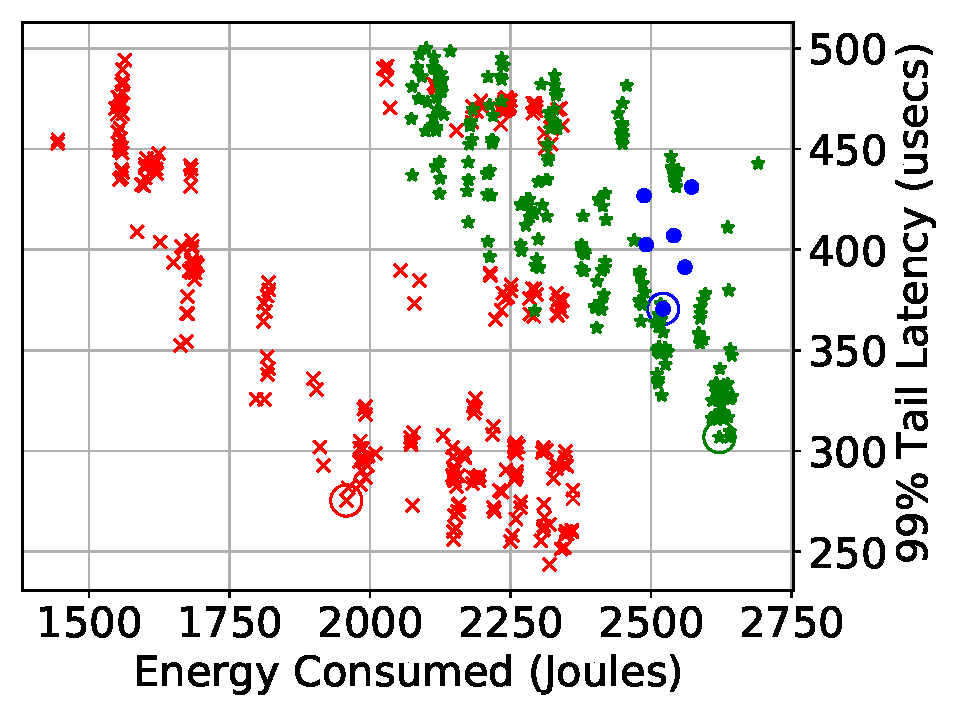
\includegraphics[width=\columnwidth]{osdi_figures/mcdsilo_200000_overview.pdf}
	\caption{MemCached Silo 200K QPS}
	\label{fig:mcdsiloov}
\end{minipage}
\end{figure*}


% super short description of 4 lines that say open versus closed and compute intensive versus simple
%We used the four network-driven workloads of Table~\ref{table:wrkcfgs} (see \cref{sec:apps} for details) to explore open and closed loop dynamics along with lower and higher application CPU requirements. 
%Open loop workloads, where one needs to meet an SLA (e.g., 99\% tail latency) under a fixed demand, tend to be common in the cloud.
%Closed-loop applications where chosen to enable us to explore scenarios where there is an interdependence between service performance and the load offered to that service.
%The range of closed versus open and degree of application processing per request provide a rich framework to expose and analyze the behavior of the operating systems. 


%Each experiment has been run using both a general-purpose OS (Linux) and an application-specific libOS and repeated across a broad sweep of values for three hardware setting: 1) Network Interface Card (NIC) Interrupt delay (ITR), 2) Dynamic Voltage and Frequency Scaling (DVFS) and 3) Running Average Power Limit (RAPL).

%In our study we compare  Linux and libOS with various static values for the three hardware settings to default Linux.  
%To understand both the impact of the settings, and where possible the cause, we built infrastructure in both systems  to collect detailed time series log data on every network interrupt; this data includes a high-precision timestamp, joules consumed, instructions and cycles executed, sleep states entered, last-level cache misses, and bytes received and transmitted.

%Across all four workloads, we ran multiple runs of a variety of different loads (Table~\ref{table:wrkcfgs}) with different values of the three hardware settings. 
%As we found areas of interest, or unexplained behavior, we added experiments.
%The results in this paper includes data from tens of thousands of experiments each with detailed logs.
%thereby composing a dataset that contains thousands of experimental runs.
%Figures~\ref{fig:netpipe8Kov}-~\ref{fig:mcdsiloov} illustrate four of the energy-performance landscapes we observed; where performance is either the total time to run the experiment for closed loop experiments, or 99\&  

%Figures~\ref{fig:netpipe8Kov}-~\ref{fig:mcdsiloov} are landscape plots that show the energy versus performance of the four workloads for one of the offered load/scenario.
%%These energy-performance landscapes can be evaluated from two perspectives; 1) identification of "best" performance and energy states and 2) exposure of how the software and hardware broadly react to sweeping the parameters explored in the two OSes.
%Each point in these graphs represents the results of an experimental run.
%Using the log from each run, we calculate the total energy consumed along with a workload-specific measure.
%In the case of netpipe and node.js workloads, the workload-specific measure we use is the time taken to complete some fixed number of sequential transactions in a closed-loop setting.
%For netpipe (figure~\ref{fig:netpipe8Kov}), we measure the time taken to complete approximately 200,000 8Kb message round-trips between a client and server configured with the same OS and hardware settings.
%For Node.JS (figure ~\ref{fig:nodejsov}), we measure the time required to serve 200,000 requests for a minimal static webpage.

%In the case of the open-loop workloads, Memcached and Memcached-Silo, we report the 99\% tail latency experienced while under a specific load of some number of queries-per-second (QPS) for a period of 20 seconds.
%Specifically, for Memcached (figure~\ref{fig:itr_figure}), we apply an offered load of 600 QPS generated using the ETC Facebook benchmark~\cite{mutilate}.
%For Memcached-Silo (figure~\ref{fig:mcdsiloov}), we apply a load of 200 QPS.
%Note that, in both open-loop cases, the offered loads are close-to but do not exceed the system's capacity.
%Furthermore, we filter any results that do not satisfy an SLA of 500 $\micro s$.  
%Each experimental run uses a unique setting for the three hardware settings we study (ITR, DVFS, and RAPL) with each of the two OSs we consider.
%We do not modify the OSs nor do we modify application software beyond choosing for Linux what is considered a production-quality configuration.

%Given that we use total time for a fixed amount of work in the close loop settings and we use 99\% tail latency in the open loop settings as performance metrics, better in all cases is indicated by a lower value.  
%Best performance and energy states thus form a pareto-optimal energy-performance curve of points that are closest to the origin in the landscape plots.  


We decided to focus our study on three hardware settings (see \cref{sec:knobs}) and four workloads (\cref{sec:apps}) that explore both closed and open loop behavior along with both high and low application processing demands.  
We compare the performance of default Linux running the workloads under the 11 scenarios in Table~\ref{table:wrkcfgs} to  Linux and libOS with a wide range of static values for the three hardware settings.  
In both systems, we build infrastructure to collect detailed time series log data on every network interrupt; this data includes a high-precision timestamp, joules consumed, instructions and cycles executed, sleep states entered, last-level cache misses, and bytes received and transmitted.
The results in this paper includes data from tens of thousands of experiments each with detailed logs.
Figures~\ref{fig:netpipe8Kov}-~\ref{fig:mcdsiloov} show example landscape plots that summarize many experiments, where each point shows performance versus energy consumed for a single experiment.  
Best performance and energy states form a pareto-optimal energy-performance curve of points that are closest to the origin in these plots.  

The relative value of one point versus another in the landscape plots depends on what value/utility one places on the importance/cost of energy versus performance.  To enable analysis,  independent of such relative value, we at times will use the product of  Energy and Performance  (EPP), as a single quantity ($Joules \times Performance$) to rank points.  
EPP is one simple way of comparing individual results as points with lower EPP represent a systems ability to achieve a better fixed points in the tradeoff space.   

Our analysis demonstrates  a number of  results, that while expected, have never been shown quantitatively: 
\begin{description}
\item[Library OS benefits] Running a single dedicated application with a Library OS structure results in significant pareto-optimal energy-performance benefits.  Specifically we found tuning the three hardware parameters we consider, with an application specific library OS stack, resulted in X-Y\% EPP improvements over the best results obtained tuning a general purpose OS (Linux) configured to run the same application in a dedicated fashion.
\item[Tuning benefits] Static tuning of the three hardware parameters resulted in significant improvements in the energy-performance behaviour of the general purpose OS, when running a dedicated application.   We observe X-Y\% EPP improvements when tuning Linux versus its default behaviours with the workloads (where its default is responsible for dynamically controlling the two of the settings). Moreover, we find that generally the statically tuned operating systems have much less variability than the default dynamic policies.
\item[Exploitable Energy-performance] Broadly we see that both OS's have a relatively clear energy-performance pareto-optimal curve that arises and identifies the settings for which there exists energy performance tradeoffs that can be exploited.
%todo: clean up next sentance, or cut  
A system with only one point with at a lower EPP may not be as useful as a system that has many distinct points at similar EPP; such points allow tuning for one's utility and cost or adjust to changes in utility and costs . 
\end{description}
  
We have developed four questions to organize and distill the surprising phenomena that arose in our study.  We will refer back to these questions as we analyze and discuss the results of our experiments. 
\subsection{Organizing Questions}
\label{sec:questions}
\paragraph{Q1} 
\label{sec:q1}
What if any impact does OS path length have on the energy consumption?
\paragraph{Q2}
\label{sec:Q2}
What if any impact does low-level OS behaviour have on the net efficiency when executing an application dominated software stack? 
Does the OS have a net effect on application code IPC?
\paragraph{Q3} 
\label{sec:Q3}
In what ways does the OS software adapt to exploit idle periods in network processing to save energy?
\paragraph{Q4}
\label{sec:Q4}
Is there an interdependence between the achievable energy-performance profile and the OS software complete
Can simplify energy management with a simpler OS?

Are their benefits to a simpler OS that enable the use of simpler strategies for setting the hardware energy parameters?

Is there a tradeoff in OS complexity and energy management setting that can be exploited to make both easier?
Can you design and implement an OS such that controlling the hardware energy management settings is easier or can compensate for a simpler implementation? 





%3) interaction between different settings is subtle, and it is critical to consider them together. 

The rest of the the paper is organized as follows: Section

